
%% bare_conf.tex
%% V1.3
%% 2007/01/11
%% by Michael Shell
%% See:
%% http://www.michaelshell.org/
%% for current contact information.
%%
%% This is a skeleton file demonstrating the use of IEEEtran.cls
%% (requires IEEEtran.cls version 1.7 or later) with an IEEE conference paper.
%%
%% Support sites:
%% http://www.michaelshell.org/tex/ieeetran/
%% http://www.ctan.org/tex-archive/macros/latex/contrib/IEEEtran/
%% and
%% http://www.ieee.org/

%%*************************************************************************
%% Legal Notice:
%% This code is offered as-is without any warranty either expressed or
%% implied; without even the implied warranty of MERCHANTABILITY or
%% FITNESS FOR A PARTICULAR PURPOSE! 
%% User assumes all risk.
%% In no event shall IEEE or any contributor to this code be liable for
%% any damages or losses, including, but not limited to, incidental,
%% consequential, or any other damages, resulting from the use or misuse
%% of any information contained here.
%%
%% All comments are the opinions of their respective authors and are not
%% necessarily endorsed by the IEEE.
%%
%% This work is distributed under the LaTeX Project Public License (LPPL)
%% ( http://www.latex-project.org/ ) version 1.3, and may be freely used,
%% distributed and modified. A copy of the LPPL, version 1.3, is included
%% in the base LaTeX documentation of all distributions of LaTeX released
%% 2003/12/01 or later.
%% Retain all contribution notices and credits.
%% ** Modified files should be clearly indicated as such, including  **
%% ** renaming them and changing author support contact information. **
%%
%% File list of work: IEEEtran.cls, IEEEtran_HOWTO.pdf, bare_adv.tex,
%%                    bare_conf.tex, bare_jrnl.tex, bare_jrnl_compsoc.tex
%%*************************************************************************

% *** Authors should verify (and, if needed, correct) their LaTeX system  ***
% *** with the testflow diagnostic prior to trusting their LaTeX platform ***
% *** with production work. IEEE's font choices can trigger bugs that do  ***
% *** not appear when using other class files.                            ***
% The testflow support page is at:
% http://www.michaelshell.org/tex/testflow/



% Note that the a4paper option is mainly intended so that authors in
% countries using A4 can easily print to A4 and see how their papers will
% look in print - the typesetting of the document will not typically be
% affected with changes in paper size (but the bottom and side margins will).
% Use the testflow package mentioned above to verify correct handling of
% both paper sizes by the user's LaTeX system.
%
% Also note that the "draftcls" or "draftclsnofoot", not "draft", option
% should be used if it is desired that the figures are to be displayed in
% draft mode.
%
\documentclass[10pt, conference, compsocconf]{IEEEtran}
% Add the compsocconf option for Computer Society conferences.
%
% If IEEEtran.cls has not been installed into the LaTeX system files,
% manually specify the path to it like:
% \documentclass[conference]{../sty/IEEEtran}





% Some very useful LaTeX packages include:
% (uncomment the ones you want to load)


% *** MISC UTILITY PACKAGES ***
%
%\usepackage{ifpdf}
% Heiko Oberdiek's ifpdf.sty is very useful if you need conditional
% compilation based on whether the output is pdf or dvi.
% usage:
% \ifpdf
%   % pdf code
% \else
%   % dvi code
% \fi
% The latest version of ifpdf.sty can be obtained from:
% http://www.ctan.org/tex-archive/macros/latex/contrib/oberdiek/
% Also, note that IEEEtran.cls V1.7 and later provides a builtin
% \ifCLASSINFOpdf conditional that works the same way.
% When switching from latex to pdflatex and vice-versa, the compiler may
% have to be run twice to clear warning/error messages.






% *** CITATION PACKAGES ***
%
%\usepackage{cite}
% cite.sty was written by Donald Arseneau
% V1.6 and later of IEEEtran pre-defines the format of the cite.sty package
% \cite{} output to follow that of IEEE. Loading the cite package will
% result in citation numbers being automatically sorted and properly
% "compressed/ranged". e.g., [1], [9], [2], [7], [5], [6] without using
% cite.sty will become [1], [2], [5]--[7], [9] using cite.sty. cite.sty's
% \cite will automatically add leading space, if needed. Use cite.sty's
% noadjust option (cite.sty V3.8 and later) if you want to turn this off.
% cite.sty is already installed on most LaTeX systems. Be sure and use
% version 4.0 (2003-05-27) and later if using hyperref.sty. cite.sty does
% not currently provide for hyperlinked citations.
% The latest version can be obtained at:
% http://www.ctan.org/tex-archive/macros/latex/contrib/cite/
% The documentation is contained in the cite.sty file itself.






% *** GRAPHICS RELATED PACKAGES ***
%
\ifCLASSINFOpdf
  % \usepackage[pdftex]{graphicx}
  % declare the path(s) where your graphic files are
  % \graphicspath{{../pdf/}{../jpeg/}}
  % and their extensions so you won't have to specify these with
  % every instance of \includegraphics
  % \DeclareGraphicsExtensions{.pdf,.jpeg,.png}
\else
  % or other class option (dvipsone, dvipdf, if not using dvips). graphicx
  % will default to the driver specified in the system graphics.cfg if no
  % driver is specified.
  % \usepackage[dvips]{graphicx}
  % declare the path(s) where your graphic files are
  % \graphicspath{{../eps/}}
  % and their extensions so you won't have to specify these with
  % every instance of \includegraphics
  % \DeclareGraphicsExtensions{.eps}
\fi
% graphicx was written by David Carlisle and Sebastian Rahtz. It is
% required if you want graphics, photos, etc. graphicx.sty is already
% installed on most LaTeX systems. The latest version and documentation can
% be obtained at: 
% http://www.ctan.org/tex-archive/macros/latex/required/graphics/
% Another good source of documentation is "Using Imported Graphics in
% LaTeX2e" by Keith Reckdahl which can be found as epslatex.ps or
% epslatex.pdf at: http://www.ctan.org/tex-archive/info/
%
% latex, and pdflatex in dvi mode, support graphics in encapsulated
% postscript (.eps) format. pdflatex in pdf mode supports graphics
% in .pdf, .jpeg, .png and .mps (metapost) formats. Users should ensure
% that all non-photo figures use a vector format (.eps, .pdf, .mps) and
% not a bitmapped formats (.jpeg, .png). IEEE frowns on bitmapped formats
% which can result in "jaggedy"/blurry rendering of lines and letters as
% well as large increases in file sizes.
%
% You can find documentation about the pdfTeX application at:
% http://www.tug.org/applications/pdftex





% *** MATH PACKAGES ***
%
%\usepackage[cmex10]{amsmath}
% A popular package from the American Mathematical Society that provides
% many useful and powerful commands for dealing with mathematics. If using
% it, be sure to load this package with the cmex10 option to ensure that
% only type 1 fonts will utilized at all point sizes. Without this option,
% it is possible that some math symbols, particularly those within
% footnotes, will be rendered in bitmap form which will result in a
% document that can not be IEEE Xplore compliant!
%
% Also, note that the amsmath package sets \interdisplaylinepenalty to 10000
% thus preventing page breaks from occurring within multiline equations. Use:
%\interdisplaylinepenalty=2500
% after loading amsmath to restore such page breaks as IEEEtran.cls normally
% does. amsmath.sty is already installed on most LaTeX systems. The latest
% version and documentation can be obtained at:
% http://www.ctan.org/tex-archive/macros/latex/required/amslatex/math/





% *** SPECIALIZED LIST PACKAGES ***
%
%\usepackage{algorithmic}
% algorithmic.sty was written by Peter Williams and Rogerio Brito.
% This package provides an algorithmic environment fo describing algorithms.
% You can use the algorithmic environment in-text or within a figure
% environment to provide for a floating algorithm. Do NOT use the algorithm
% floating environment provided by algorithm.sty (by the same authors) or
% algorithm2e.sty (by Christophe Fiorio) as IEEE does not use dedicated
% algorithm float types and packages that provide these will not provide
% correct IEEE style captions. The latest version and documentation of
% algorithmic.sty can be obtained at:
% http://www.ctan.org/tex-archive/macros/latex/contrib/algorithms/
% There is also a support site at:
% http://algorithms.berlios.de/index.html
% Also of interest may be the (relatively newer and more customizable)
% algorithmicx.sty package by Szasz Janos:
% http://www.ctan.org/tex-archive/macros/latex/contrib/algorithmicx/




% *** ALIGNMENT PACKAGES ***
%
%\usepackage{array}
% Frank Mittelbach's and David Carlisle's array.sty patches and improves
% the standard LaTeX2e array and tabular environments to provide better
% appearance and additional user controls. As the default LaTeX2e table
% generation code is lacking to the point of almost being broken with
% respect to the quality of the end results, all users are strongly
% advised to use an enhanced (at the very least that provided by array.sty)
% set of table tools. array.sty is already installed on most systems. The
% latest version and documentation can be obtained at:
% http://www.ctan.org/tex-archive/macros/latex/required/tools/


%\usepackage{mdwmath}
%\usepackage{mdwtab}
% Also highly recommended is Mark Wooding's extremely powerful MDW tools,
% especially mdwmath.sty and mdwtab.sty which are used to format equations
% and tables, respectively. The MDWtools set is already installed on most
% LaTeX systems. The lastest version and documentation is available at:
% http://www.ctan.org/tex-archive/macros/latex/contrib/mdwtools/


% IEEEtran contains the IEEEeqnarray family of commands that can be used to
% generate multiline equations as well as matrices, tables, etc., of high
% quality.


%\usepackage{eqparbox}
% Also of notable interest is Scott Pakin's eqparbox package for creating
% (automatically sized) equal width boxes - aka "natural width parboxes".
% Available at:
% http://www.ctan.org/tex-archive/macros/latex/contrib/eqparbox/





% *** SUBFIGURE PACKAGES ***
%\usepackage[tight,footnotesize]{subfigure}
% subfigure.sty was written by Steven Douglas Cochran. This package makes it
% easy to put subfigures in your figures. e.g., "Figure 1a and 1b". For IEEE
% work, it is a good idea to load it with the tight package option to reduce
% the amount of white space around the subfigures. subfigure.sty is already
% installed on most LaTeX systems. The latest version and documentation can
% be obtained at:
% http://www.ctan.org/tex-archive/obsolete/macros/latex/contrib/subfigure/
% subfigure.sty has been superceeded by subfig.sty.



%\usepackage[caption=false]{caption}
%\usepackage[font=footnotesize]{subfig}
% subfig.sty, also written by Steven Douglas Cochran, is the modern
% replacement for subfigure.sty. However, subfig.sty requires and
% automatically loads Axel Sommerfeldt's caption.sty which will override
% IEEEtran.cls handling of captions and this will result in nonIEEE style
% figure/table captions. To prevent this problem, be sure and preload
% caption.sty with its "caption=false" package option. This is will preserve
% IEEEtran.cls handing of captions. Version 1.3 (2005/06/28) and later 
% (recommended due to many improvements over 1.2) of subfig.sty supports
% the caption=false option directly:
%\usepackage[caption=false,font=footnotesize]{subfig}
%
% The latest version and documentation can be obtained at:
% http://www.ctan.org/tex-archive/macros/latex/contrib/subfig/
% The latest version and documentation of caption.sty can be obtained at:
% http://www.ctan.org/tex-archive/macros/latex/contrib/caption/




% *** FLOAT PACKAGES ***
%
\usepackage{fixltx2e}
% fixltx2e, the successor to the earlier fix2col.sty, was written by
% Frank Mittelbach and David Carlisle. This package corrects a few problems
% in the LaTeX2e kernel, the most notable of which is that in current
% LaTeX2e releases, the ordering of single and double column floats is not
% guaranteed to be preserved. Thus, an unpatched LaTeX2e can allow a
% single column figure to be placed prior to an earlier double column
% figure. The latest version and documentation can be found at:
% http://www.ctan.org/tex-archive/macros/latex/base/



%\usepackage{stfloats}
% stfloats.sty was written by Sigitas Tolusis. This package gives LaTeX2e
% the ability to do double column floats at the bottom of the page as well
% as the top. (e.g., "\begin{figure*}[!b]" is not normally possible in
% LaTeX2e). It also provides a command:
%\fnbelowfloat
% to enable the placement of footnotes below bottom floats (the standard
% LaTeX2e kernel puts them above bottom floats). This is an invasive package
% which rewrites many portions of the LaTeX2e float routines. It may not work
% with other packages that modify the LaTeX2e float routines. The latest
% version and documentation can be obtained at:
% http://www.ctan.org/tex-archive/macros/latex/contrib/sttools/
% Documentation is contained in the stfloats.sty comments as well as in the
% presfull.pdf file. Do not use the stfloats baselinefloat ability as IEEE
% does not allow \baselineskip to stretch. Authors submitting work to the
% IEEE should note that IEEE rarely uses double column equations and
% that authors should try to avoid such use. Do not be tempted to use the
% cuted.sty or midfloat.sty packages (also by Sigitas Tolusis) as IEEE does
% not format its papers in such ways.





% *** PDF, URL AND HYPERLINK PACKAGES ***
%
%\usepackage{url}
% url.sty was written by Donald Arseneau. It provides better support for
% handling and breaking URLs. url.sty is already installed on most LaTeX
% systems. The latest version can be obtained at:
% http://www.ctan.org/tex-archive/macros/latex/contrib/misc/
% Read the url.sty source comments for usage information. Basically,
% \url{my_url_here}.



% *** Do not adjust lengths that control margins, column widths, etc. ***
% *** Do not use packages that alter fonts (such as pslatex).         ***
% There should be no need to do such things with IEEEtran.cls V1.6 and later.
% (Unless specifically asked to do so by the journal or conference you plan
% to submit to, of


% correct bad hyphenation here
%\hyphenation{op-tical net-works semi-conduc-tor}
\usepackage{epsfig}
\usepackage{defs}
\usepackage{amsmath}
\usepackage{amsthm}
\usepackage{amssymb}
\usepackage{algorithm}
\usepackage{algorithmic}
\usepackage{comment}
\usepackage{verbatim}
\usepackage{dcolumn}
\newcolumntype{d}[1]{D{.}{.}{#1}}


\begin{document}
%
% paper title
% can use linebreaks \\ within to get better formatting as desired
\title{Scalable Overlapping Community Detection}


% author names and affiliations
% use a multiple column layout for up to two different
% affiliations

%\author{
%\IEEEauthorblockN{Ismail El-Helw}
%\IEEEauthorblockA{Department of Computer Science\\
%Vrije Universiteit Amsterdam\\
%The Netherlands\\
%ielhelw@cs.vu.nl}
%\and
%\IEEEauthorblockN{Rutger Hofman}
%\IEEEauthorblockA{Department of Computer Science\\
%Vrije Universiteit Amsterdam\\
%The Netherlands\\
%rutger@cs.vu.nl}
%\and
%\IEEEauthorblockN{Henri Bal}
%\IEEEauthorblockA{Department of Computer Science\\
%Vrije Universiteit Amsterdam\\
%The Netherlands\\
%bal@cs.vu.nl}
%}

\author{\IEEEauthorblockN{Ismail El-Helw\IEEEauthorrefmark{1},
Rutger Hofman\IEEEauthorrefmark{1},
Wenzhe Li\IEEEauthorrefmark{2},
Sungjin Ahn\IEEEauthorrefmark{3},
Max Welling\IEEEauthorrefmark{4} and
Henri Bal\IEEEauthorrefmark{1}}
\IEEEauthorblockA{\IEEEauthorrefmark{1}Vrije Universiteit Amsterdam, The Netherlands\\ Email: \{ielhelw,rutger,bal\}@cs.vu.nl}
\IEEEauthorblockA{\IEEEauthorrefmark{2}University of Southern California, USA\\ Email: wenzheli@usc.edu}
\IEEEauthorblockA{\IEEEauthorrefmark{3}University of Montreal, Canada \\ Email: sungjia@ics.uci.edu}
\IEEEauthorblockA{\IEEEauthorrefmark{4}University of Amsterdam, The Netherlands\\ Email: m.welling@uva.nl}}

% conference papers do not typically use \thanks and this command
% is locked out in conference mode. If really needed, such as for
% the acknowledgment of grants, issue a \IEEEoverridecommandlockouts
% after \documentclass

% for over three affiliations, or if they all won't fit within the width
% of the page, use this alternative format:
% 
%\author{\IEEEauthorblockN{Michael Shell\IEEEauthorrefmark{1},
%Homer Simpson\IEEEauthorrefmark{2},
%James Kirk\IEEEauthorrefmark{3}, 
%Montgomery Scott\IEEEauthorrefmark{3} and
%Eldon Tyrell\IEEEauthorrefmark{4}}
%\IEEEauthorblockA{\IEEEauthorrefmark{1}School of Electrical and Computer Engineering\\
%Georgia Institute of Technology,
%Atlanta, Georgia 30332--0250\\ Email: see http://www.michaelshell.org/contact.html}
%\IEEEauthorblockA{\IEEEauthorrefmark{2}Twentieth Century Fox, Springfield, USA\\
%Email: homer@thesimpsons.com}
%\IEEEauthorblockA{\IEEEauthorrefmark{3}Starfleet Academy, San Francisco, California 96678-2391\\
%Telephone: (800) 555--1212, Fax: (888) 555--1212}
%\IEEEauthorblockA{\IEEEauthorrefmark{4}Tyrell Inc., 123 Replicant Street, Los Angeles, California 90210--4321}}




% use for special paper notices
%\IEEEspecialpapernotice{(Invited Paper)}




% make the title area
\maketitle

\begin{abstract}
  % 1. what is the field of your work?
% 2. what is the problem you solve?
% 3. what is your solution/approach?
% 4. what are your results?
%
Recent advancements in machine learning algorithms have transformed the data
analytics domain and provided innovative solutions to inherently difficult
problems. However, training models at scale over large data sets remains a
daunting challenge. One such problem is the detection of overlapping
communities within graphs. For example, a social network can be modeled as a
graph where the vertices and edges represent individuals and their
relationships. As opposed to the problem graph partitioning or clustering, an
individual can be part of multiple communities which significantly increases
the problem complexity.
In this paper, we present and evaluate an efficient parallel and
distributed implementation of a Stochastic Gradient Markov Chain Monte Carlo
algorithm that solves the overlapping community detection problem. We show that
the algorithm can scale and process graphs consisting of billions of edges and
tens of millions of vertices on a compute cluster of 65 nodes. To the best of
our knowledge, this is the first time that the problem of deducing overlapping
communities has been learned for problems of such a large scale.


\end{abstract}

\begin{IEEEkeywords}
Distributed computing; Parallel programming; High performance computing; Performance analysis; Machine learning;
\end{IEEEkeywords}


\IEEEpeerreviewmaketitle

\section{Introduction}
The tremendous amount of data that we generate through our daily applications such as social networking services, online shopping, and news recommendations, provides us with an opportunity to extract hidden but invaluable and useful information. Realizing this opportunity, however, requires a significant amount of effort because traditional machine learning algorithms often become extremely inefficient with large amounts of data.

There have been two main approaches to this end; machine learning researchers have developed new scalable algorithms~\cite{bottou2010large, boyd2011distributed} while systems and networking researchers have worked on developing new generic infrastructure systems which can be leveraged to construct machine learning algorithms more efficiently~\cite{dean2008mapreduce, chang2008bigtable}. However, it is clear that, in most cases we see the best performance by carefully integrating both of these approaches in one system.

One such big data problem is analyzing large graphs such as social networks where it is not unusual to see a network consisting of billions of edges and tens of million of vertices~\cite{yang2015defining}. In particular, we are interested in the overlapping community detection problem~\cite{xie2013overlapping}, where the goal is to learn the probability distribution of each vertex to participate in each community, provided a set of vertices, the link information between them (which is usually very sparse), and the number of latent communities. A community can be seen as a densely connected group of vertices that are only sparsely connect to the rest of the network. 

This problem is modeled by the mixed membership stochastic blockmodels (MMSB)~\cite{airoldi2009mixed} and in this paper we are particularly interested in a variant of the MMSB, called assortative-MMSB (a-MMSB\footnote{Although we work on a-MMSB for simplicity, it is also straightforward to apply the proposed method to the general MMSB model.}) \cite{gopalan2012scalable}.

The MMSB model is a probabilistic graphical model~\cite{koller2009probabilistic} that represents a convenient paradigm for modeling complex relationships between a potentially large number of random variables. Bayesian graphical models, where we define priors and infer posteriors over parameters also allow us to quantify model uncertainty and facilitate model selection and averaging. However, an increasingly urgent question is whether these models and their inference procedures will be up to the challenge of handling very large graphs.

There have been two main recent advances in this direction of scalable Bayesian inference methods based on stochastic variational Bayes (SVB)~\cite{hoffman2013stochastic,gopalan2013efficient,gopalan2012scalable} and stochastic gradient Markov chain Monte Carlo (SG-MCMC)~\cite{welling2011bayesian,patterson2013stochastic,ahn2014distributed,ahn2012bayesian}. Both methods have the important property that they only require a small subset of the data for every iteration. In other words, they can be applied to (infinite) streaming data.

In this paper, we are particularly interested in the SG-MCMC method applied to the a-MMSB model introduced in \cite{LiAW15}, which turned out to be faster and more accurate than the SVB method. Although \cite{LiAW15} proposed a scalable algorithm for the problem, there is still room to improve the performance further by considering a custom high-performance implementation. To this end, we propose a design of a parallel and distributed system specifically tailored to solve the a-MMSB problem. In particular, we use a mixture of OpenMP, MPI and RDMA in order to efficiently scale and accelerate the algorithm's computation.

Achieving this goal necessitated overcoming several challenges. First, the algorithm's state grows rapidly with larger graphs and number of latent communities. Since the full state information is too large to fit in a single machine's memory, it is partitioned and distributed across a cluster of machines. Second, to access the full state, each cluster node must read remote memory hosted by its peers. We leveraged RDMA to limit the high latency of such operations and increase the communication bandwidth. To reduce the latency further, we pipelined the algorithms computations such that data can be fetched in advance over the network. Finally, the algorithm's computation had to be effectively distributed across the cluster nodes and parallelized further within each node to exploit their multi-core CPUs.

The remainder of this paper is organized as follows. Section~2 provides and overview of the algorithm and its theoretical foundation. The design and implementation of the parallel and distributed solution is presented in Section~3. Section~4 evaluates the efficacy of the system and analyzes its performance. Finally, Section~5 provides concluding remarks.

% -------\\
% Community detection is the central problem in network analysis, with the goal of identifying the groups of related nodes that are densely connected within this group but sparsely connected to the rest of the network. Different from classical community detection problem where we assume each node belongs to one single community, our paper considers overlapping communities where each of the nodes might belong to multiple communities. In particular, we consider the model called a-MMSB(Assortive Mixed Membership Stochastic Blockmodel) in this paper, which was first introduced in~\cite{gopalan2012scalable}.\\


% a-MMSB, as a probabilistic graphical model, represents a convenient paradigm for modeling complex relationships between a potentially large number of random variables. It also uses priors and posteriors to quantify model uncertainty and facilitate model selection and averaging. While a-MMSB provides rich representation power, like other Bayesian models, the inference procedures of handling big data which is common in real world is still a very challenging problem. \\



% Consider the large networks such as a social network, it easily runs into billions of edges and tens of million of nodes. In addition to that, the number of communities might exceed few millions. 
% There were two types of scalable algorithm for a-MMSB have been introduced recently \cite{gopalan2012scalable}, stochastic variational Bayesian inference (SVB) and stochastic gradient Markov chain Monte Carlo(SG-MCMC), respectively. Both methods have the important property that each iteration only relies on a small subset of the data. Although both methods can work for some large networks with many hundreds of nodes, the performance is far less satisfactory when it applies to the so-called "big data" such as facebook network with millions of nodes and billions of edges. Given the facts that \cite{LiAW15}, SG-MCMC runs faster and converges to the better local minima, in this paper, we mainly consider the problem of scaling up SG-MCMC to the big data set.  \textit{As far as we know, this is the first paper that studies community detection on the frencter dataset with few billion's of edges.}





\section{Background}
% In this section, we briefly review the Bayesian model we are considering in this paper.

% In this section, we briefly review the Bayesian model we are considering in this paper.
\subsection{Assortative Mixed-membership Stochastic Blockmodels (a-MMSB)}
The assortative mixed membership stochastic blockmodel (a-MMSB) ~\cite{gopalan2012scalable} is a special case of MMSB~\cite{airoldi2009mixed} that models the group-structure in a network of $N$ vertices. Consider a set  $\cV^*$ containing all the vertices in the graph, and a set $\cE^*$ containing all the linked edges between pairs of vertices. Each vertex $a$ in the vertex set $\cV^*$ has a $K$-dimension probability distribution $\pi_a$ of participating in the $K$ members of the community set $\cK$.  For every possible peer $b$ in the network, each vertex $a$ randomly draws a community $z_{ab}$. If a pair of vertices ($a,b$) in the edge set $\cE^*$ are in the same community, i.e., $z_{ab}=z_{ba} = k$, then they have a significant probability $\bt_k$ to connect, i.e., $y_{ab}=1$. Otherwise this probability is small. Each community has its connection strength $\beta_{k} \in (0,1)$ which explains how likely its members are linked to each other. The whole generative process of a-MMSB is then described by,
\benum
\item For each community $k$, draw community strength $\bt_k \sim \mbox{Beta}(\eta)$
\item For each vertex $a$, draw community memberships $\pi_a \sim \mbox{Dirichlet}(\al)$
\item For each pair of vertices $a$ and $b$,
\benum
	\item Draw interaction indicator $z_{ab} \sim \pi_a$
    \item Draw interaction indicator $z_{ba} \sim \pi_b$
    \item Draw link $y_{ab} \sim \mbox{Bernoulli}(r)$, where $r = \bt_k$ if $z_{ab}=z_{ba}=k$, and $r=\dt$ otherwise.
\eenum
\eenum

\subsection{Stochastic Gradient Markov Chain Monte Carlo}
The algorithm we are working on in this paper is based on the stochastic gradient Langevin dynamics (SGLD) ~\cite{welling2011bayesian}. SLGD applies the following update rule to obtain samples from a posterior distribution $p(\ta|\cX) \propto p(\cX|\ta) p(\ta)$ of $N$ i.i.d. data points $\cX=\{x_i\}_{i=1}^{N}$:
\bea
\ta^* \law \ta + \f{\epsilon_t}{2}\left(\nabla_{\ta}\log p(\ta_t)+N\bar{g}(\ta;\cD_n)\right) + \xi_t, \label{eqn:sgld_update}
\eea
where $\xi_t \sim \cN(0,\epsilon_t )$ with $\ep_t$ the step size, $\cD_n$ a minibatch of size $n$ sampled from $\cX$, and $\bar{g}(\ta;\cD_n)$ the mean stochastic gradient, i.e., $\frac{1}{|\cD_n|}\sum_{x\in \cD_n}^{}\grad_{\ta} \log p(x|\ta)$. As the step size goes to zero by a schedule satisfying $\sm{t}{\infty}\ep_t = \infty$ and $\sm{t}{\infty}\ep_t^2 < \infty$, SGLD samples from the true posterior distribution. One benefit of using SGLD is that we do not need the Metropolis-Hastings (MH) accept-reject tests since the rejection probability goes to zero as the step size collapses to zero. Although the finite step size, which we use in practice rather than converging to zero, still results in some bias, we can reduce the overall error by drawing many more samples per unit time. 

SGLD originated from the Langevin Monte Carlo (LMC)~\cite{girolami2011riemann}, where unlike SGLD the gradient is computed exactly by using all data points. Then, Metropolis-Hastings accept-reject tests are applied. Comparing to LMC, SGLD only requires to process a minibatch $\cD_n$ at each iteration and ignores the MH test, and thus the computational complexity substantially reduces from $\cO(N)$ to $\cO(n)$.   

The stochastic gradient Riemannian Langevin dynamics (SGRLD)~\cite{patterson2013stochastic} is a subclass of SGLD which is developed to efficiently sample from the probability simplex. By applying Riemannian geometry~\cite{girolami2011riemann} and using the minibatch-based estimator in Eqn. \ref{eqn:sgld_update}, it achieved the state-of-the-art performance for latent Dirichlet allocation (LDA)~\cite{blei2003latent}. In particular, for a $K$-dimensional probability simplex $\pi$, it uses the \textit{expanded-mean} re-parameterization trick, where the probability of a category $k$ is given by $\pi_k = \ta_k / \sum_{j=1}^K \ta_j$ with $\ta_k \sim \text{Gamma}(\al,1)$ and $\al$ a hyperparameter of the Dirichlet distribution $p(\pi | \al )$. Then, the update rule of SGRLD is:
\bea
\ta_{k}^* \law \left| \ta_{k} + \f{\ep_t}{2} \left( \al - \ta_{k} + \f{N}{|\cD_n|} \sum_{d \in \cD_n} g_d(\ta_{k}) \right) + (\ta_{k})^\ha \xi_{t} \right|. \label{eqn:sgrld_update}
\eea
here $g_d(\ta_{k})$ is the gradient of the log posterior w.r.t. $\ta_{k}$ on a data point $d\in \cD_n$.


\subsection{Scalable MCMC for a-MMSB}
This section describes the SG-MCMC algorithm for a-MMSB. Please refer \cite{LiAW15} for more details. The algorithm iterates updating local parameter $\pi$ and a global parameter $\beta$. Since both parameters lie on the probability simplex, SGRLD is applied to make the sampling process more efficient. Here, the parameters $\phi$ and $\ta$ are used to re-parameterize $\pi$ and $\beta$ respectively. After updating $\phi$ and $\ta$, we can obtain $\pi$ and $\beta$ by normalizing $\phi$ and $\ta$, respectively. In the following, we briefly sketch the iterative update steps.

\paragraph{\textbf{Sampling global parameters}} The update rule for global parameter $\theta$ is
\bea
\ta_{ki}^* \law \left| \ta_{ki} + \f{\ep}{2} \left\{ \eta - \ta_{ki} + h(\cE_{n_t})\sum_{(a,b) \in \cE_{n_t}}g_{ab}(\ta_{ki})\right\} \right.\nn \\ \left.+ (\ta_{ki})^{\ha}\xi_{ki} \right|, \label{eqn:global_update}
\eea
where 
\bea
g_{ab}(\ta_{ki})
&=& \f{f_{ab}^{(y)}(k,k)}{Z_{ab}^{(y)}} \left(\f{|1-i-y|}{\ta_{ki}} - \f{1}{\ta_k} \right).
\eea
here $\cE_{n_t}$ is a mini-batch of $n_t$ vertex pairs sampled from $\cE^*$, and $h(\cE_{n_t})$ is the weighting terms and 
\bea
f_{ab}^{(y)}(k,l)=
\begin{cases}
\bt_k^y(1-\bt_k)^{(1-y)}\pi_{ak}\pi_{bk}, & \mbox{if } k=l\\
\dt^{y}(1-\dt)^{(1-y)} \pi_{ak} \pi_{bl}, & \mbox{if } k \neq l \nn
\end{cases}
\label{eqn:case}
\eea
$Z_{ab}^{(y)}$ is the normalization constant which we can compute in $\cO(K)$ time \cite{LiAW15}.

\paragraph{\textbf{Sampling local parameters}}
The update rule for the local parameters $\phi$ is
\bea
\phi_{ak}^* \law \left| \phi_{ak} + \f{\ep}{2} \left( \al - \phi_{ak} + \f{N}{|\cV_n|} \sum_{b \in \cV_n} g_{ab}(\phi_{ak})\right) \right. \nn \\ \left. + (\phi_{ak})^{\ha} \xi_{ak}\right|.\label{eqn:local_update}
\eea
where \bea
g_{ab}(\phi_{ak}) = \f{f_{ab}^{(y)}(k)}{Z_{ab}^{(y)}\phi_{ak}} - \f{1}{\phi_a}.
\eea
Here, the $\cV_n$ is a random mini-batch of $n$ vertices sampled from $\cV^*$. Note that $|\cV_n| \ll |\cV^*|=N$.

The overall pseudo-code of the sequential algorithm is described in Algorithm 1. 

\begin{algorithm}[t]
\caption{Sequential version of SG-MCMC for a-MMSB}\label{alg}
\begin{algorithmic}[1]
\STATE Initialize $\pi , \bt, \phi, \ta$
\WHILE {sampling}
\STATE Sample a mini-batch of vertex pairs, $\cE_t$, from $E$
\FOR {each vertex in $\cE_t$}
	\STATE Sample a mini-batch of vertices, $\cV_t$, from $V$
    \STATE Update $\phi_{a}$ using Eqn~\ref{eqn:local_update}
  %  $\phi_{a}^* \law \left| \phi_{a} + \f{\ep_{\phi}}{2} \left( \al - \phi_{a} + \f{N}{|\cV_t|} \sum_{b \in \cV_t} G_{\phi_{a}}\right) + (\phi_{a})^{\ha} \xi_{a}\right|$
    \STATE Obtain $\pi_a$ from $\phi_a^*$ \ENDFOR
\FOR {$k = 1,\dots,K$}
    \STATE Update $\ta_{k}$ using Eqn~\ref{eqn:global_update}
   % $\ta_{k}^* \law \left| \ta_{k} + \f{\ep_\ta}{2} \left( \eta - \ta_{k} + h(\cE_t) \sum_{(a,b) \in \cE_t} G_{\ta_{k}}(a,b) \right) + (\ta_{k})^{\ha}\xi_{k} \right|$
    \STATE Obtain $\bt_k$ from $\ta_k^*$
\ENDFOR
\ENDWHILE
\end{algorithmic}
\end{algorithm}


\begin{comment}
Assortative mixed-membership stochastic blockmodel (a-MMSB) [1] is a special case of MMSB [8] that models the group-structure in a network of $N$ nodes. In particular, each node $a$ in the node set $\cV^*$ has a $K$-dimension probability distribution $\pi_a$ of participating in the $K$ members of the community set $\cK$. For every possible peer $b$ in the network, each node $a$ randomly draws a community $z_{ab}$. If a pair of nodes ($a,b$) in the edge set $\cE^*$ are in the same community: $z_{ab}=z_{ba} = k$, then they have a significant probability $\bt_k$ to connect, i.e., $y_{ab}=1$. Otherwise this probability is small. Each community has its connection strength $\beta_{k} \in (0,1)$ which explains how likely its members are linked to each other.  

The generative process of a-MMSB is then given by,

\benum
\item For each community $k$, draw community strength $\bt_k \sim \mbox{Beta}(\eta)$
\item For each node $a$, draw community memberships $\pi_a \sim \mbox{Dirichlet}(\al)$
\item For each pair of nodes $a$ and $b$,
\benum
	\item Draw interaction indicator $z_{ab} \sim \pi_a$
    \item Draw interaction indicator $z_{ba} \sim \pi_b$
    \item Draw link $y_{ab} \sim \mbox{Bernoulli}(r)$, where $r = \bt_k$ if $z_{ab}=z_{ba}=k$, and $r=\dt$ otherwise.
\eenum
\eenum

Unlike the a-MMSB, the original MMSB maintains pair-wise community strength $\bt_{k,k'}$ for all pairs of the communities. Note that it is trivial to extend the results that we obtain in this paper to the general MMSB model. The joint probability of the above process can be written as:
\begin{align}
p(y,z,\pi ,\bt | \al, \eta) &= \prod_{a=1}^{N} \prod_{b > a}^{N} p(y_{ab} | z_{ab}, z_{ba}, \bt) p(z_{ab}|\pi_a)\nonumber \\ &p(z_{ba}|\pi_b) \pd{a}{N}p(\pi_a|\al) \pd{k}{K} p(\bt_k|\eta).\label{eqn:joint}
\end{align}

Both variational inference [1,4,16] and collapsed Gibbs sampling algorithms [11] have been used successfully for small to medium scale problems. However, the $\cO(N^2)$ computational complexity per update prevents it from being applied to large scale networks. A stochastic variational algorithm was developed in [1] to address this issue, where each update only depends on a small mini-batch of the nodes in the network. 


%%%%%%%%%%%%%%%%%%%%%%%%%%%%%%%%%%%%%%%%%%%%%%%%%%%%%%%%%%%%%%%
\section{Stochastic Gradient MCMC Algorithms}
Our algorithm will be based on the stochastic gradient Langevin dynamics (SGLD) [3]. To sample from a posterior distribution $p(\ta|\cX) \propto p(\cX|\ta) p(\ta)$ given $N$ i.i.d. data points $\cX=\{x_i\}_{i=1}^{N}$, SGLD applies the following update rule:
\bea
\ta^* \law \ta + \f{\epsilon_t}{2}\left(\nabla_{\ta}\log p(\ta_t)+N\bar{g}(\ta;\cD_n)\right) + \xi, \label{eqn:sgld_update}
\eea
where $\xi \sim \cN(0,\epsilon_t )$ with $\ep_t$ the step size, $\cD_n$ a mini-batch of size $n$ sampled from $\cX$, and $\bar{g}(\ta;\cD_n) = \frac{1}{|\cD_n|}\sum_{x\in \cD_n}^{}\grad_{\ta} \log p(x|\ta)$. As the step size goes to zero by a schedule satisfying $\sm{t}{\infty}\ep_t = \infty$ and $\sm{t}{\infty}\ep_t^2 < \infty$, SGLD samples from the true posterior distribution. In SGLD, the Metropolis-Hastings (MH) accept-reject tests are ignored since the rejection probability goes to zero as the step size collapses to zero. While for a finite step size this results in some bias, the overall error is reduced by the reduction of variance due to the ability to draw many more samples per unit time. 

SGLD originated from the Langevin Monte Carlo (LMC) [15] where, unlike SGLD, the gradient is computed exactly using all data points and then a Metropolis-Hastings accept-reject test is applied. Because at each iteration SGLD requires to process only a mini-batch $\cD_n$ and ignores the MH test, the computation complexity per iteration is only $\cO(n)$ as opposed to $\cO(N)$ of LMC. Any mini-batch sampling algorithm in the form of Eqn. \eqref{eqn:sgld_update} is called valid SGLD as long as it guarantees the gradient estimator to be unbiased, i.e.,
$\eE_{\cD_n} \left[N\bar{g}(\ta;\cD_n)\right] = \grad_{\ta} \log p(\cX|\ta)\label{eqn:sgld_grad_estm}$ and the variance to be finite [5].

%%%%%%%%%%%%%%
%\subsection{Stochastic Gradient Riemannian Langevin Dynamics (SGRLD)}

The stochastic gradient Riemannian Langevin dynamics (SGRLD) [2] is a subclass of SGLD which is developed to sample from the probability simplex. By applying Riemannian geometry [15] and using the mini-batch estimator in Eqn. \ref{eqn:sgld_update}, it achieved the state-of-the-art performance for latent Dirichlet allocation (LDA). In particular, for a $K$-dimensional probability simplex $\pi$, it uses the \textit{expanded-mean} re-parameterization trick, where the probability of a category $k$ is given by $\pi_k = \ta_k / \sum_{j=1}^K \ta_j$ with $\ta_k \sim \text{Gamma}(\al,1)$ and $\al$ a hyperparameter of the Dirichlet distribution $p(\pi | \al )$.
Then, the update rule becomes

%==============================================================

\bea
\ta_{k}^* \law \left| \ta_{k} + \f{\ep}{2} \left( \al - \ta_{k} + \f{N}{|\cD_n|} \sum_{d \in \cD_n} g_d(\ta_{k}) \right) + (\ta_{k})^\ha \xi_{} \right|. \label{eqn:sgrld_update}
\eea
here $g_d(\ta_{k})$ is the gradient of the log posterior w.r.t. $\ta_{k}$ on a data point $d\in \cD_n$.



%%%%%%%%%%%%%%%%%%%%%%%%%%%%%%%%%%%%%%%%%%%%%%%%%%%%%%%%%%%%%%%
\section{Scalable MCMC for a-MMSB}
Our algorithm iterates updating local parameters $\pi$ and a global parameter $\beta$. Because both parameters lie on the probability simplex, we start from the SGRLD and modify it to be more efficient. Also, we introduce parameters $\phi$ and $\ta$ to re-parameterize $\pi$ and $\beta$ respectively. Thus, we alternatingly sample in the $\phi$ and $\ta$ spaces, and then obtain $\pi$ and $\beta$ by normalizing $\phi$ and $\ta$. From Eqn. \ref{eqn:joint}, summing over the latent variable $z$, we obtain the following joint probability,
\bea
&p(y, \pi , \bt | \al , \eta) = \prod_{a} p(\pi_a | \al ) + \prod_{a} p(\bt_k | \eta)\nn \\
&+ \prod_{a} \prod_{b > a}\sum_{z_{ab}, z_{ba}} p(y_{ab}, z_{ab}, z_{ba} | \bt , \pi_a, \pi_b)
\label{eqn:log_joint}.
\eea


%==============================================================
\subsection{Sampling the global parameter}

By the re-parameterization, we have $\beta_k=\ta_{k1}/(\ta_{k0}+\ta_{k1})$, where $\ta_{ki}\sim$ Gamma$(\eta)\propto \ta_{ki}^{\eta-1}e^{-\ta_{ki}}$. Because $p(y, \pi , \bt | \al , \eta)$ decomposes into $p(y,\bt|\pi,\eta) p(\pi|\al)$, replacing $\bt$ by $\ta$, we compute the derivative of log of Eqn. \ref{eqn:log_joint} w.r.t. $\ta_{ki}$ for $i=\{0,1\}$ as follows:
\bea
\fp{\ln p(y ,\ta | \pi, \eta )}{\ta_{ki}} =
\fp{}{\ta_{ki}} \ln p(\ta_{ki} | \eta) + \sum_{a}\sum_{b>a} g_{ab}(\ta_{ki}),
\label{eqn:grad_bt}
\eea
where $g_{ab}(\ta_{ki}) = \fp{}{\ta_{ki}} \ln \sum_{z_{ab},z_{ba}} p(y_{ab},z_{ab},z_{ba} | \ta , \pi_a, \pi_b)$ which, similar to SGRLD for LDA [2], we can rewrite as
\bea
g_{ab}(\ta_{ki}) = \eE \left[ \eI[z_{ab}=z_{ba}=k] \left( \f{|1-i-y_{ab}|}{\ta_{ki}} - \f{1}{\ta_{k}} \right)\right]. \label{eqn:G}
\eea
where $\ta_{k}=\sum_i \ta_{ki}$ and $\eI[S]$ is equal to $1$ if a condition $S$ is TRUE and $0$ otherwise. The expectation is w.r.t. the posterior distribution of latent variables $z_{ab}$ and $z_{ba}$,
\bea
&&p(z_{ab}=k,z_{ba}=l | y_{ab}, \pi_a, \pi_b, \bt )\\ &&\propto f_{ab}^{(y)}(k,l)=
\begin{cases}
\bt_k^y(1-\bt_k)^{(1-y)}\pi_{ak}\pi_{bk}, & \mbox{if } k=l\\
\dt^{y}(1-\dt)^{(1-y)} \pi_{ak} \pi_{bl}, & \mbox{if } k \neq l \nn
\end{cases}
\label{eqn:case}
\eea
here we used simple notation $y$ instead of $y_{ab}$. Unlike the SGRLD for LDA [2], we compute the expectation in Eqn. \eqref{eqn:G} analytically by computing the normalization constant $Z_{ab}^{(y)} = \sm{k}{K}\sm{l}{K} f_{ab}^{(y)}(k,l)$ which can be reduced to $\cO(K)$ computation as follows
\begin{align}
&Z_{ab}^{(y)} = \dt^{y}(1-\dt)^{(1-y)} \nonumber\\&+\sm{k}{K} \left( \bt_k^{y}(1-\bt_k)^{(1-y)} - \dt^{y}(1-\dt)^{(1-y)}\right)\pi_{ak}\pi_{bk}
\end{align}

Then Eqn. \eqref{eqn:G} becomes
\bea
g_{ab}(\ta_{ki}) 
&=& \f{f_{ab}^{(y)}(k,k)}{Z_{ab}^{(y)}} \left(\f{|1-i-y|}{\ta_{ki}} - \f{1}{\ta_k} \right).
\eea
Plugging this into Eqn. \ref{eqn:sgrld_update}, we obtain the update rule for the global parameter,

\bea
\ta_{ki}^* \law \left| \ta_{ki} + \f{\ep}{2} \left\{ \eta - \ta_{ki} + h(\cE_{n_t})\sum_{(a,b) \in \cE_{n_t}}g_{ab}(\ta_{ki})\right\} \right.\nn \\ \left.+ (\ta_{ki})^{\ha}\xi_{ki} \right|, \label{eqn:global_update}
\eea
here $\cE_{n_t}$ is a mini-batch of $n_t$ node pairs sampled from $\cE^*$ for which we use the following strategy.

\textbf{Stratified sampling:} considering that the number of links is much smaller than that of non-links, we can reduce the variance of the gradient using stratified sampling, similar to the method used in [1]. For this, at every iteration we first randomly select a node $a$ and then toss a coin with probability 0.5 to decide whether to sample link edges or non-link edges for node $a$. If it is a link, we assign all of the link edges of node $a$ to $\cE_{n_t}$. Otherwise, i.e. if it is non-link, we uniformly sample a mini-batch of $N/m$ non-link edges from the entire set of non-link edges and assign it to $\cE_{n_t}$. Here, the $m$ is a hyper-parameter. Note that the size of $|\cE_{n_t}|$ will thus be much smaller than the total number of $N(N-1)/2$ edges when $m$ is reasonably large. Then, to ensure that the gradient is unbiased, a \textit{scaling parameter} $h(\cE_{n_t})$ is multiplied. Specifically, $h(\cE_{n_t})$ is set to $N$ when $\cE_{n_t}$ is a set of link edges and to $mN$ otherwise. 

Because the global parameters $\{\beta_k\}$ does not change very fast compared to the local parameters $\{\pi_{ak}\}$, in practice we update only a random subset of the $\{\beta_k\}$ at each iteration.

\subsection{Sampling the local parameters}

Similar to the global parameter, we re-parameterize the local parameter $\pi_a$ such that $\pi_{ak} = \phi_{ak} / \sum_{j=1}^{K}\phi_{aj}$, with $\phi_{ak}\sim$ Gamma$(\alpha)\propto \phi_{ak}^{\alpha-1}e^{-\phi_{ak}}$. Then, taking the derivative of the log of Eqn. \ref{eqn:log_joint} w.r.t. $\phi_{ak}$, we obtain
\bea
\fp{\ln p(y , \phi | \bt, \al)}{\phi_{ak}} = \fp{}{\phi_{ak}} \ln p(\phi_{ak} | \al) +
\sum_{b} g_{ab}(\phi_{ak})
\eea
where $g_{ab}(\phi_{ak}) = \fp{}{\phi_{ak}} \ln \sum_{z_{ab}, z_{ba}} p(y_{ab}, z_{ab}, z_{ba} | \bt , \phi_a, \phi_b)$ which can be written as 
\bea 
g_{ab}(\phi_{ak}) = \eE\left[ \f{\eI [z_{ab} = k]}{ \phi_{ak}} - \f{1}{\phi_{a\cdot}} \right].
\label{eqn:grad_local}
\eea
Here the expectation is w.r.t. the distribution in Eqn. \eqref{eqn:case}. To compute the expectation analytically, we first integrate out $z_{ba}$ from Eqn. \eqref{eqn:case} because the expectation depends only on $z_{ab}$, and obtain the following probability up to a normalization constant

\begin{align}
&f_{ab}^{(y)}(k) = \sum_{l=1}^K f_{ab}^{(y)}(k,l)\nonumber \\ =& \pi_{ak}
\left\{ \bt_k^{y}(1-\bt_k)^{(1-y)} \pi_{bk} + \dt^{y}(1-\dt)^{(1-y)} (1- \pi_{bk}) \right\}.\label{eqn:local_f}
\end{align}

Then we obtain the normalization term by $Z_{ab}^{(y)} = \sm{k}{K}f_{ab}^{(y)}(k)$. 
Integrating out the expectation in Eqn. \eqref{eqn:grad_local}, we obtain 
\bea
g_{ab}(\phi_{ak}) = \f{f_{ab}^{(y)}(k)}{Z_{ab}^{(y)}\phi_{ak}} - \f{1}{\phi_a}.
\eea 
Plugging this to Eqn. \ref{eqn:sgrld_update}, we obtain the SGRLD update rule for the local parameter $\phi_{ak}$
\bea
\phi_{ak}^* \law \left| \phi_{ak} + \f{\ep}{2} \left( \al - \phi_{ak} + \f{N}{|\cV_n|} \sum_{b \in \cV_n} g_{ab}(\phi_{ak})\right) \right. \nn \\ \left. + (\phi_{ak})^{\ha} \xi_{ak}\right|.\label{eqn:local_update}
\eea
Here, the $\cV_n$ is a random mini-batch of $n$ nodes sampled from $\cV^*$. Note that $|\cV_n| \ll |\cV^*|=N$.

\end{comment}

\section{System Design}
\label{design-section}

\begin{comment}
- distributed parallelisation:
  cut up into stages like the CC-Grid paper:
  pipeline:
    1) sample mini-batch
    2) sample neighbors
    3) update_phi
  4) update_pi
  5) update_theta
  5a) calc_grads
  5b) sum_grads
  5c) update_theta
  6) update_beta
  7) perplexity

- DKV RDMA store

- data dependencies:
  mb = nodes in the mini-batch
  nb = nodes in the neighbor sets
  H  = held-out set

  	pi	phi	beta	theta	grad.th	G	prev.mini-batch
  1) 	-	-	-	-		R	-
  2) 	-	-	-	-		R	R
  3) 	R(mb)	R	R	-		R	-
	R(nb)
  4)	R/W(mb)	R	-	-		-	-
  5a)	R(mb)	-	R	R	W	-	-
  5b)	-	-	-	-	R/W	-	-
  5c)	-	-	-	R/W	R	-	-
  6)	-	-	W	R	-	-	-
  7)	R(H)	-	R(H)	-	-	H	-

- parallelization:
  1) sequential at master's, multithreaded
  2) parallel over mb; at workers', multithreaded
  3) parallel over mb; at workers', multithreaded
  4) parallel over mb; at workers', multithreaded
  5a) parallel at workers', multithreaded
  5b) omp_reduce(+) at workers', MPI reduce global
  5c) at master's, multithreaded
  6) broadcast theta by master, parallel update at workers'
  7) parallel over H; at workers', multithreaded
     reduce(+) at workers, MPI reduce global

- distributed parallelization:
  trade memory size for communication costs
  pity: the algorithm is already memory-dominant

- synchronization:
  in principle, each step synchronized
  but: pipelining in sample mini-batch / load pi/phi / update_phi

- data sizes:
  G has N vertices and |E| undirected edges
  |H| is 1..10% of |E|
  pi, phi, beta, theta are float32
  pi[N][K + 1] if phi folded into pi
  beta[K]
  theta[K][2]
  so, pi is the memory eater
   . beta/theta are replicated
   . phi is folded into pi
   . pi is partitioned across the workers
  G is stored at the master only: save the memory for pi so we can handle
  larger K. The relevant slices of G (m's adjacency lists) are scattered
  together with the mini-batch.
  G is stored as a Google SparseHash because c++ std::(unordered_)set has a
  huge overhead per item. Workers unpack their slice of G into a
  std::unordered_set because that is somewhat faster.

- pi storage: DKV
   . pi/phi is read in 3), 4), 5a), 7)
   . pi is written in 4); read[i], then write[i], so no other data dependencies
   . so access is very synchronous: either read-only, or write without
     concurrent readers
   . DKV store properties:
      - single-sized keys
      - contiguous key space (integers 0..N-1)
      - update-only writes: no new KVs, no deletes
     so: no load imbalance, no hashing that is worth its name
      - no read/write or write/write concurrency
     so:
      - build RDMA store with remote reads and remote writes only, with exactly
        one RDMA transaction per read or write
\end{comment}

% rationale -- here or in the intro?

% http://stanford.edu/~rezab/nips2014workshop/slides/jure.pdf

The SG-MCMC algorithm described in the previous section has an abundance of
opportunities for parallelism, for the multi-threaded, shared-memory type as
well as for distributed-memory parallelism. The benefit of multi-threaded
parallelism is speed-up of the computation. A distributed implementation
additionally allows to store data in the collective memory of the cluster
machine and increases memory bandwidth which scales with the number of
machines. The downside of a distributed implementation is that it requires
considerably more programming effort.

% intro parallelisation, distribution

This section describes how we parallelize the algorithm.
In most places, the usage of multi-threaded parallelism
is straightforward, therefore, we will discuss details only where appropriate. The
distributed design follows a master-worker paradigm, where in essence
the master controls the parallel operations and the workers perform the
calculations. For thread parallelism, we annotate the program with
OpenMP~\cite{OpenMPSpec}. For distributed communication, we use
MPI~\cite{Forum:1994:MMI:898758}.

% largest data structures

\subsection{Data distribution}

As is common in machine learning problems, the edges of the graph are divided
into two sets, a training set $G$ and a held-out set $\cE_h$.
The largest data structures of the algorithm are $G$, $\cE_h$, $\pi$ and~$\phi$.
For the largest dataset in this paper, com-Friendster, $G$ has 1.8~billion
undirected edges. In our representation with directed edges, this takes
up 13.5GB. Our design lets $G$ reside only at the master. We observe that
the calculations in the update stages only require the subset of $G$ that
is touched by the mini-batch vertices, so the master scatters that subset to
the workers together with the scattering of the mini-batch vertices. This way,
we trade a reduction in memory at the workers against the cost of limited
communication. In contrast, $\cE_h$ can be partitioned statically over all
machines for the parallel perplexity calculation.

$\pi$~and $\phi$ are 32-bit float arrays of size $K \times N$. For our
largest distributed experiment, com-Friendster with $N$=64M and $K$=12K, each
requires~3TB. We decided to store only $\pi$ and $\pi^{sum}$, and recalculate
$\phi$ from these whenever appropriate. Here, we trade a substantial reduction
in memory against limited computation. $\pi$ is partitioned across the workers,
and $\pi$ values are accessed via a DKV (distributed key-value) store.

% lack of locality

The distribution within the graph of the vertices of the mini-batch as well as
the neighbor sets is completely random. That means that there is no locality
in $\pi$ access patterns, especially in the accesses to the neighbor sets
$\cV_t$.
Hence, there is no opportunity to exploit caching of $\pi$ through data
locality.

% each of the stages

\subsection{Implementation of distributed parallelism}

This section describes the parallelization of each of the stages of the
algorithm's main loop. All but the first stage justify parallelization for
high values of combinations of the  parameters $|\cV_n|$, $K$, $\cV_t$, and $|\cE_h|$.

The first stage, mini-batch selection (line 3 in Algorithm~1), is done at the master and it is
not itself parallelized. However, the distributed implementation overlaps
its execution using pipeline parallelism while the workers are
performing \textit{update\_phi}. The mini-batch is partitioned equally over
the workers and the relevant sections of $G$ are distributed together with the
mini-batch subsets.

After a worker has received its subset of the mini-batch, it samples a neighbor
set $\cV_t$ for each of its mini-batch vertices, using thread parallelism
(line 5 in Algorithm~1).

The next stage, \textit{update\_phi} (line 6 in Algorithm~1), is the algorithm's dominant stage, not
only in calculation but also in memory accesses. It performs $M\times n\times
K$ operations. It can be fully parallelized because it is a data-parallel
operation over each of the mini-batch vertices. \textit{update\_phi} loads the
$\pi$ values for the local mini-batch vertices and their neighbors from the
DKV store. The updates to $\phi$ for the mini-batch vertices are calculated
independently using thread parallelism.

These updates are used by \textit{update\_pi} (line 7 in Algorithm~1) locally, besides the value of
$\pi/\phi$ for the mini-batch vertices. The update to $\pi$ requires $M\times
K$ operations, and it is done in parallel over mini-batch vertices. Because of
memory consistency, this stage awaits completion of \textit{update\_phi} with
an MPI barrier. After the calculation, the updated values of $\pi+\pi^{sum}$
are written through the DKV store.

\textit{update\_beta} (lines 10 and 11 in Algorithm~1) requires $M\times K$ operations. It is preceded by an MPI
barrier to ensure that up-to-date $\pi$ values are read. \textit{update\_beta}
is split into four steps. The first stage partitions the mini-batch across
machines to calculate contributions to $\nabla\theta$. The values of $\pi$ for
the local mini-batch vertices are loaded from the DKV store. These calculations
are done with thread parallelism over the mini-batch vertices. In the second step,
a multi-threaded summation is performed to calculate the contributions per
machine, followed by a distributed summation using an MPI reduce operation. The
third step calculates $\beta$ from $\theta$ sequentially at the master. This
operation takes only $K$ steps. The resulting $\beta$ is broadcast with MPI
to the workers.

The calculation of perplexity requires $|\cE_h|\times K$ steps. Each of the
machines owns a subset of $\cE_h$. It loads up-to-date values of $\pi$ for each
vertex in its part of $\cE_h$, then for each of its edges in $\cE_h$ it calculates the
contribution to the perplexity using thread parallelism. The resulting
contributions are summed to the global perplexity value in two stages,
with a local OpenMP reduction followed by a global MPI reduction.

Note that the calculation requirements per iteration do not depend
on $N$ or $|E|$, the size of the network graph. However, larger graphs are
expected to require more iterations to achieve convergence.

\subsection{Pipelining of computation and loading $\pi$}

As will be shown in Section~\ref{eval-pipeline}, loading $\pi$ is the
dominant contribution within the dominant stage \textit{update\_phi}. This
is the performance bottleneck of the distributed algorithm. We introduce
pipeline parallelism in order to shorten the critical path. Loading $\pi$
and calculating \textit{update\_pi} are partitioned into chunks, so the
calculation of a chunk is overlapped with loading the next chunk of $\pi$
values, and also with sampling the mini-batch at the master and deploying
it to the workers.

\subsection{RDMA Distributed Key-Value Store}

Modern network technology allows access to the memory of remote machines
through the network cards (NICs) without involvement from the remote host
altogether~\cite{Hamada_infinibandtrade,Beck:2011:PER:2043535.2043537}.
This has opened up the development of
extremely efficient remote memory services, often in the form of DKV stores.
This project stores $\pi$ in a DKV store in the collective memory of the
cluster, where $\pi[i]+\pi^{sum}[i]$ is the value for key $i$. We decided not
to use any of the existing implementations of RDMA DKV stores, and instead
build our own DKV store on top of the Infiniband ib-verbs~API. The
main consideration is that our use case is unusually simple in a number
of important aspects. The KV layout is static in the sense that there are
no inserts or deletes after the initial population, which allows a static
partitioning of KV pairs over the machines. The values are all of the same size,
a vector of $K+1$ floats. The access pattern is well controlled because the
computation is partitioned into stages that are separated by barriers. A
stage either reads values or updates values. The algorithm ensures that updates
are always targeting unique elements,
therefore, there are no read/write or write/write hazards. The existing DKV
stores (RamCloud~\cite{Ousterhout:2015:RSS:2818727.2806887}, FaRM~\cite{179767},
and reputedly the fastest, Herd~\cite{Kalia:2014:URE:2740070.2626299}) incur
overhead for insert/delete flexibility, concurrency control, or variable-sized
values. Our use case allows us to do any operation in exactly one RDMA read
or RDMA write. Herd argues
that replacing RDMA reads by
an RPC to the server, followed by an unreliable write, is faster. However,
they show this only holds for small payload packets, up to 256B. A $\pi$
packet in our application is typically thousands to hundreds of thousands
of 4-byte floats.

\section{Evaluation}

This section presents an in-depth empirical analysis of the design discussed in
Section~\ref{design-section}. To this end, we assess the scalability and
efficiency of the solution using multiple criteria.
%
First, an evaluation of the \textit{strong scaling} behavior of the distributed
algorithm is presented.
%
Second, the \textit{weak scaling} of the solution is assessed with respect to increasing
numbers of targeted latent communities.
%
Next, the effects of \textit{pipelining the computation} and varying the number of latent communities on the system's
performance is analyzed.
%
Further, we evaluate the efficiency and overhead associated with \textit{network
communication} between cluster nodes.
%
Finally, we \textit{contrast} the effectiveness of scaling the computation horizontally
and vertically.

\begin{table*}
  \centering
  \begin{tabular}{l r r l}
    Name            & \#Vertices &       \#Edges & Description \\
    \hline
    com-LiveJournal &  3,997,962 &    34,681,189 & Online blogging social network \\
    com-Friendster  & 65,608,366 & 1,806,067,135 & Online gaming social network \\
    com-Orkut       &  3,072,441 &   117,185,083 & Online social network \\
    com-Youtube     &  1,134,890 &     2,987,624 & Video-sharing social network \\
    com-DBLP        &    317,080 &     1,049,866 & Computer science bibliography collaboration network \\
    com-Amazon      &    334,863 &       925,872 & Product co-purchasing network \\
    \hline
  \end{tabular}
  \caption{Summary of SNAP graph data sets used for evaluation.}
  \label{tab-datasets}
\end{table*}

Empirical results were obtained by performing experiments on the VU and TU/D
DAS5 clusters which consist of 68 and 48 compute nodes respectively. Each
compute node is equipped with a dual 8-core Intel Xeon E5-2630v3 CPU clocked
at 2.40GHz, 64GB of memory and 8TB of storage. Moreover, the compute nodes of
each site are interconnected by
FDR~InfiniBand. All of the experiments reported in this section utilized
publicly available graphs from the Stanford Large Network Dataset
Collection~(SNAP) \cite{snapnets}. Table~\ref{tab-datasets} lists the
collection of data sets used.

%################################################
\subsection{Strong scaling}

\begin{figure*}[t] % [htb]
  \centering
  \epsfig{file=plots/sweep-over-np-fixed-K.eps, width=\textwidth}
  \caption{(a) Execution time of 2048 algorithm iterations for the
  same problem size (com-Friendster, K=1024, M=16384 n=32) across different
  cluster sizes. (b) Speedup achieved for same experiments in (a) with respect to
  8-nodes}
  \label{fig-strong-scaling}
\end{figure*}

In order to evaluate the horizontal scalability of the distributed
implementation we tested the system's performance across different cluster
sizes while holding the problem size constant. For this study, we used the
com-Friendster graph as it contains the largest number of vertices and edges.
%
Figure~\ref{fig-strong-scaling}-a presents the execution time of 2048 algorithm
iterations across multiple cluster sizes. The x-axis starts from 8 worker nodes
as the data set is too large to fit into the collective memory of a smaller
cluster.
%
As shown in the figure, the execution
time steadily decreases by increasing the cluster size.
A deeper analysis of the individual execution phases of the algorithm provides
insights into the scalability if its building blocks.
%
In addition to the total execution time, Figure~\ref{fig-strong-scaling}-a
presents the cumulative time spent in individual computational phases across
iterations. Moreover, Figure~\ref{fig-strong-scaling}-b presents the speedup
achieved for the same experiments reported in
Figure~\ref{fig-strong-scaling}-a. As is clearly shown, the dominant phase of
the execution is update\_pi.
The reported total time for each cluster size is significantly less than the
sum of the execution times of the individual phases. This is due to the
overlapping execution of the two most expensive phases, namely, update\_pi and
deploy\_minibatch. Both of these phases initially gain significant speedup with the
addition of compute nodes. However, the speedup curve gradually slows down for
larger cluster sizes as the work granularity of each worker node decreases,
limiting their resource utilization.
%
The time spent in update\_beta remains relatively constant across cluster sizes
as it performs an insignificant amount of work compared to the synchronization
overhead of a collective MPI reduction operation contained within it.

%################################################
\subsection{Weak Scaling}

\begin{figure*}[t] % [htb]
  \centering
  
\epsfig{file=plots/sweep-over-K-proportional-np.eps, width=\textwidth}
  \caption{(a) Average execution time per algorithm iteration varying
  the number of latent communities proportionally to the number of compute
  nodes. (b) The exact number of communities used for each data point in (a).}
  \label{fig-weak-scaling}
\end{figure*}

A study of a system's weak scaling aids in the assessment of the communication
and synchronization overheads associated with the management of large clusters.
Similarly, it can expose complex issues that hinder performance at scale such
as load imbalance. To fairly evaluate the algorithm's weak scaling behavior we
conducted several executions varying the cluster size and the number of latent
communities proportionally. This methodology ensures that each compute node
performs a relatively constant amount of computational work across all
configurations. However, the number and size of messages exchanged between the
nodes would vary significantly. Figure~\ref{fig-weak-scaling}-a presents the
average execution
time per algorithm iteration across different cluster sizes. On the other hand,
Figure~\ref{fig-weak-scaling}-b reports the set number of communities for each
cluster configuration. The relative change in the average execution time per
iteration is insignificant even though the communication intensity increases
for larger cluster sizes. This observation verifies that the system's overall
overhead is minimal. Additionally, the experimental results shows that the
implementation is capable of achieving good speedups provided the input problem
is large enough for the given cluster size.

%################################################
\subsection{Pipeline efficiency}

\begin{figure}[t] % [htb]
  \centering
  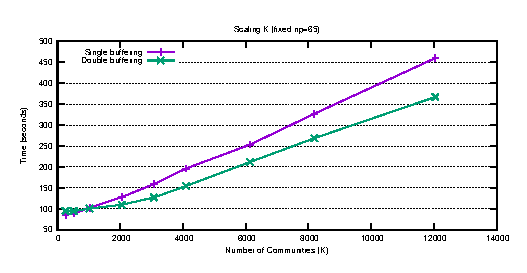
\epsfig{file=plots/sweep-over-K-fixed-np.eps, width=\columnwidth}
  \caption{Performance effect of varying the number of communities on the
    algorithm's execution time on 64-nodes when using single- or
    double-buffering.}
  \label{fig-pipeline}
\end{figure}

As discussed in Section~\ref{design-section}, the collective memory of all
worker nodes serves as the storage for the state of the computation. As such,
the rows of $\pi$ are equally and statically partitioned across all workers.
Given that $\pi$ accesses are random, a node in a cluster of size $C$ must
fetch $(C-1)/C$ of all read requests over the network. Therefore, large cluster
configurations exhibit higher bandwidth demands and are more sensitive
to network latency. To reduce the negative effects of network latency on the
computation, a pipelining scheme was devised to prefetch data dependencies.
Figure~\ref{fig-pipeline} presents the execution time of 1024 algorithm
iterations on a 64-node cluster with double-bufferring enabled and disabled.
Naturally, increasing the number of communities causes a proportional increase
in execution time. However, when double-buffering is enabled, some of the
incurred network latency is hidden by overlapping it with computation.
Moreover, since both computation time and network latency increase with larger
$K$, the benefit of pipelining increases. This can be observed through the
widening gap between both lines depicted in Figure~\ref{fig-pipeline}.

%################################################
\subsection{Horizontal vs. Vertical Scalability}
\begin{figure}[t] % [htb]
  \centering
  
\epsfig{file=plots/hpc-cloud.eps, width=\columnwidth}
  \caption{Performance comparison between the distributed implementation
  running on DAS5 and the multi-threaded solution on machine with 40-cores and
  1TB of RAM.}
  \label{fig-scale-up}
\end{figure}
One of the main drawbacks of designing a distributed solution for a given
algorithm is the inherent complexity of communication and synchronization. A
slightly simpler approach would be developing a multi-threaded version and
running it on a machine with abundant memory and CPU cores. In such a context,
access to all of the algorithm's state would be an order of magnitude faster
than RDMA. Additionally, the overhead associated with synchronizing threads is
negligible compared to using MPI primitives. To evaluate the efficacy of both
approaches we utilized SURFsara's HPC Cloud system to instantiate a virtual
machine with 40~CPU cores and 1TB of memory. The physical machine underlying
the HPC Cloud system contains 40-CPU cores and does not oversubscribe
resources. Therefore, by provisioning all 40~cores we ensured that there is no
resource contention from other users of the system. Figure~\ref{fig-scale-up}
reports the execution time per algorithm iteration for two experimental setups.
Namely, using the HPC Cloud system compared to using 64-nodes of the DAS5
cluster. Clearly, the parallel and distributed implementation vastly
outperforms the single-node multi-threaded solution. Moreover, the trajectory
of both curves shows a widening gap between them suggesting that the relative
performance difference will increase for larger $K$.
%
In conclusion, the overhead of network communication in the distributed version
is more than compensated by the increasing compute power compared to a
a single-node implementation.

%################################################
\subsection{Cluster Communication Efficiency}

%################################################
\subsection{Convergence of Large Datasets}
\begin{figure*}[t] % [htb]
  \centering
  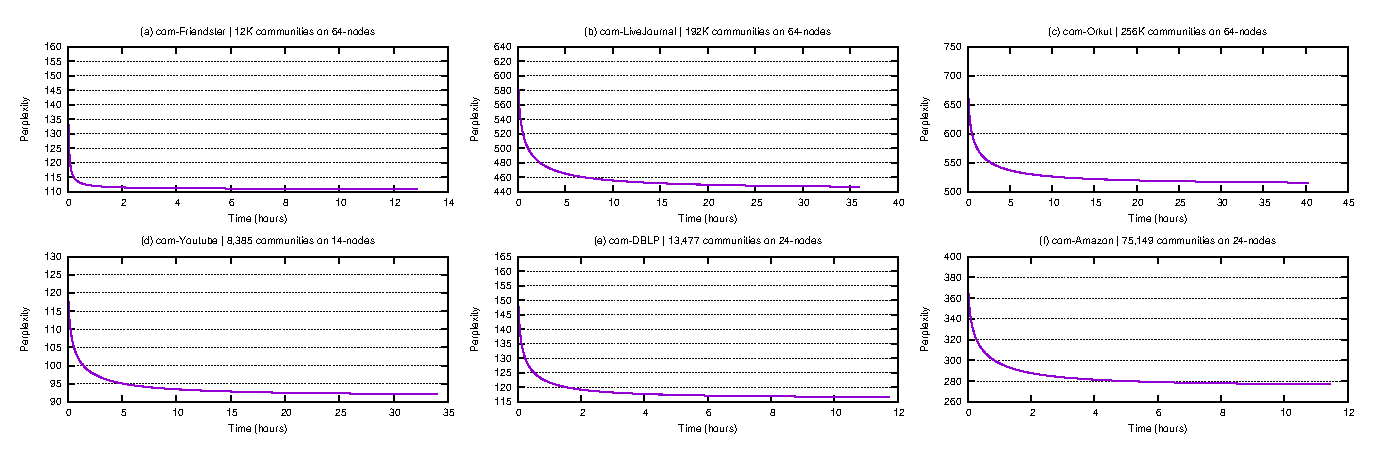
\epsfig{file=plots/ppx.eps, width=\textwidth}
  \caption{Convergence time of 6 different data sets.}
  \label{fig-ppx}
\end{figure*}

The previous sections focused on the computational performance of the
distributed implementation. However, the algorithm's throughput does not
necessarily indicate how fast it can converge to a solution. For instance, it
remains unclear how many iterations are needed for the algorithm to reach a
stable state and terminate. Therefore, we now shift our focus to the
convergence time to assess the system's utility. Figure~\ref{fig-ppx} presents
the convergence time of 6 different data sets with a diverse set of properties.




\section{Conclusion}

The recent advancements of machine learning algorithms make them ideal
candidates to solve complex problems. However, using these solutions in order
to process problems at scale is still a daunting task. In particular, knowledge
of parallel and distributed computing techniques is necessary to facilitate the
development of such systems and streamline their execution time.

In this paper, we shared our experience in developing a highly scalable and
efficient solution for a stochastic gradient Markov chain Monte Carlo algorithm
that detects overlapping communities in graphs. The system design had to
overcome several obstacles in order to achieve high performance. Specifically,
we discussed how the algorithm was structured to facilitate its
parallelization. Moreover, we evaluated the efficacy of overlapping computation
with communication to hide latency.  Further, we demonstrated the use of a
mixture of MPI and RDMA primitives to speedup the communication between cluster
nodes.

We conducted a thorough empirical evaluation of the system to study its strong
and weak scalability on 64 cluster nodes using large data sets.  Additionally,
we assessed the efficiency of the algorithm's resource utilization. Finally, a
demonstration of the implementation's utility was provided by processing 6
different organic data sets.


%\section*{Acknowledgment}
%The authors would like to thank...
%more thanks here

\bibliographystyle{IEEEtran}
% argument is your BibTeX string definitions and bibliography database(s)
\bibliography{IEEEabrv,paper}

% that's all folks
\end{document}


